\section{Marco Teórico}
  \subsection{Conceptos de Biología}

    \begin{frame}\frametitle{\textbf{Conceptos de Biología}}
    \end{frame}
    \begin{frame}\frametitle{\textbf{Conceptos de Biología}}
        \begin{center}
          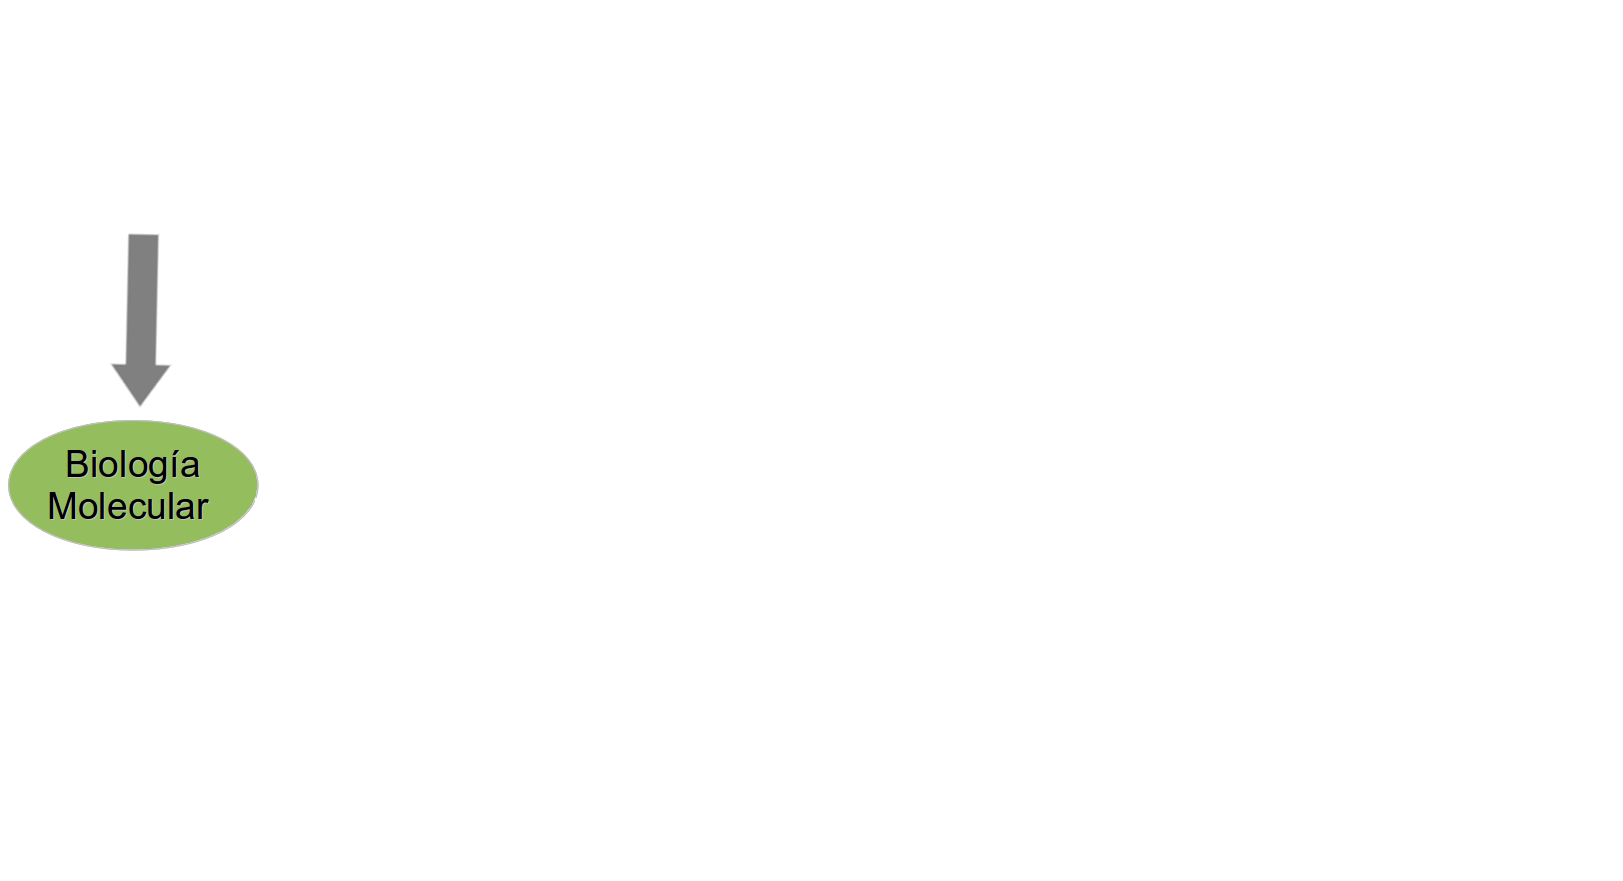
\includegraphics[scale=.2]{images/biologia1.png}
        \end{center}
    \end{frame}

    \begin{frame}\frametitle{\textbf{Conceptos de Biología}}
        \begin{center}
          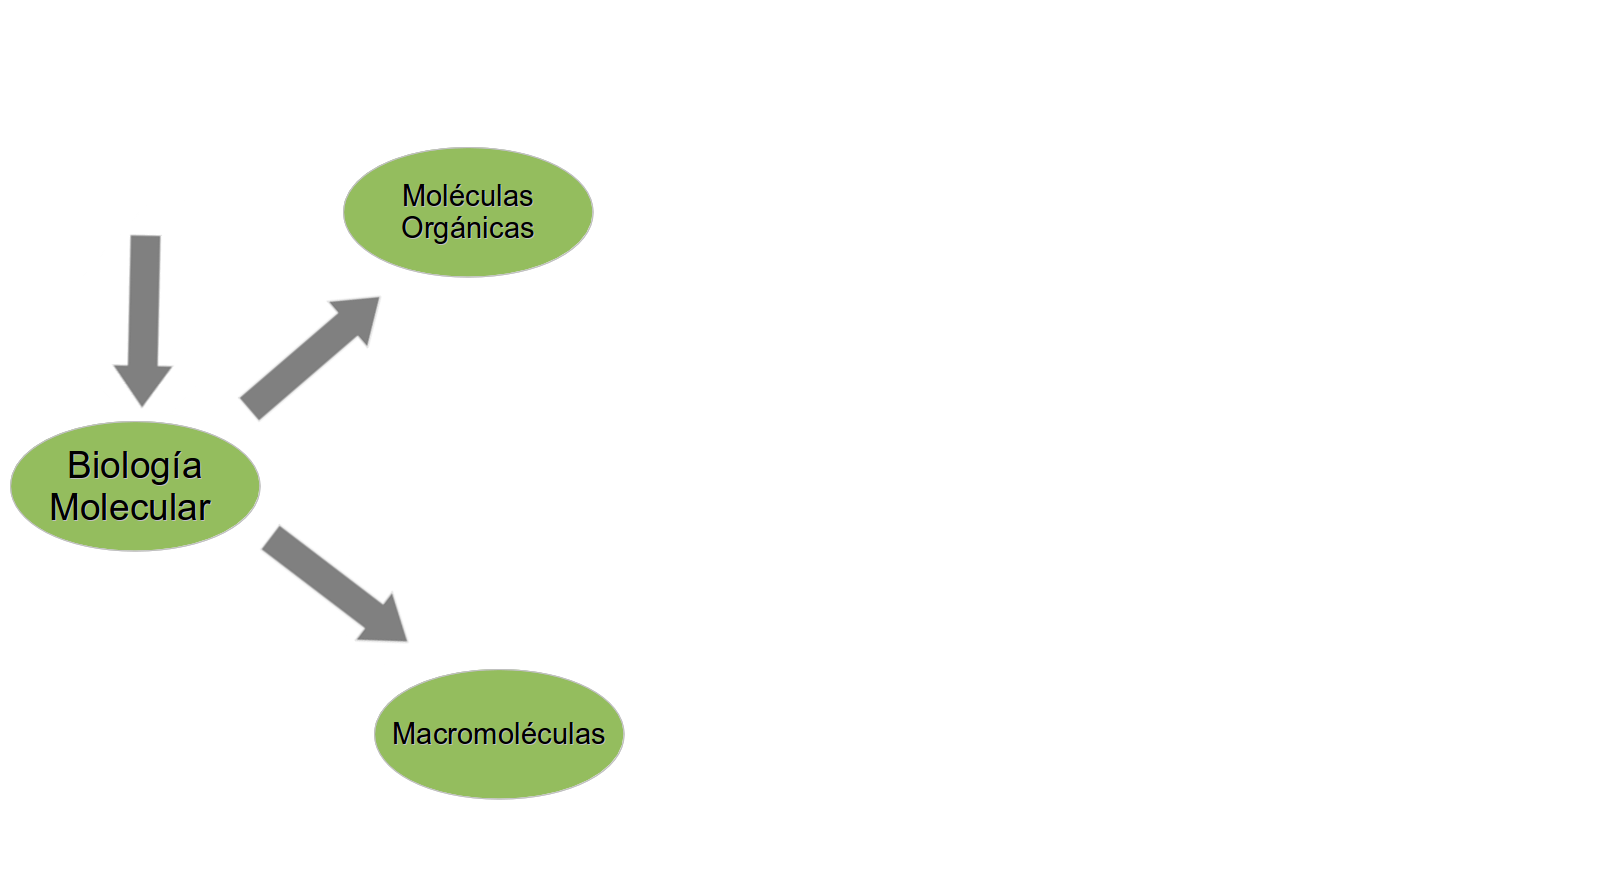
\includegraphics[scale=.2]{images/biologia2.png}
        \end{center}
    \end{frame}

    \begin{frame}\frametitle{\textbf{Conceptos de Biología}}
        \begin{center}
          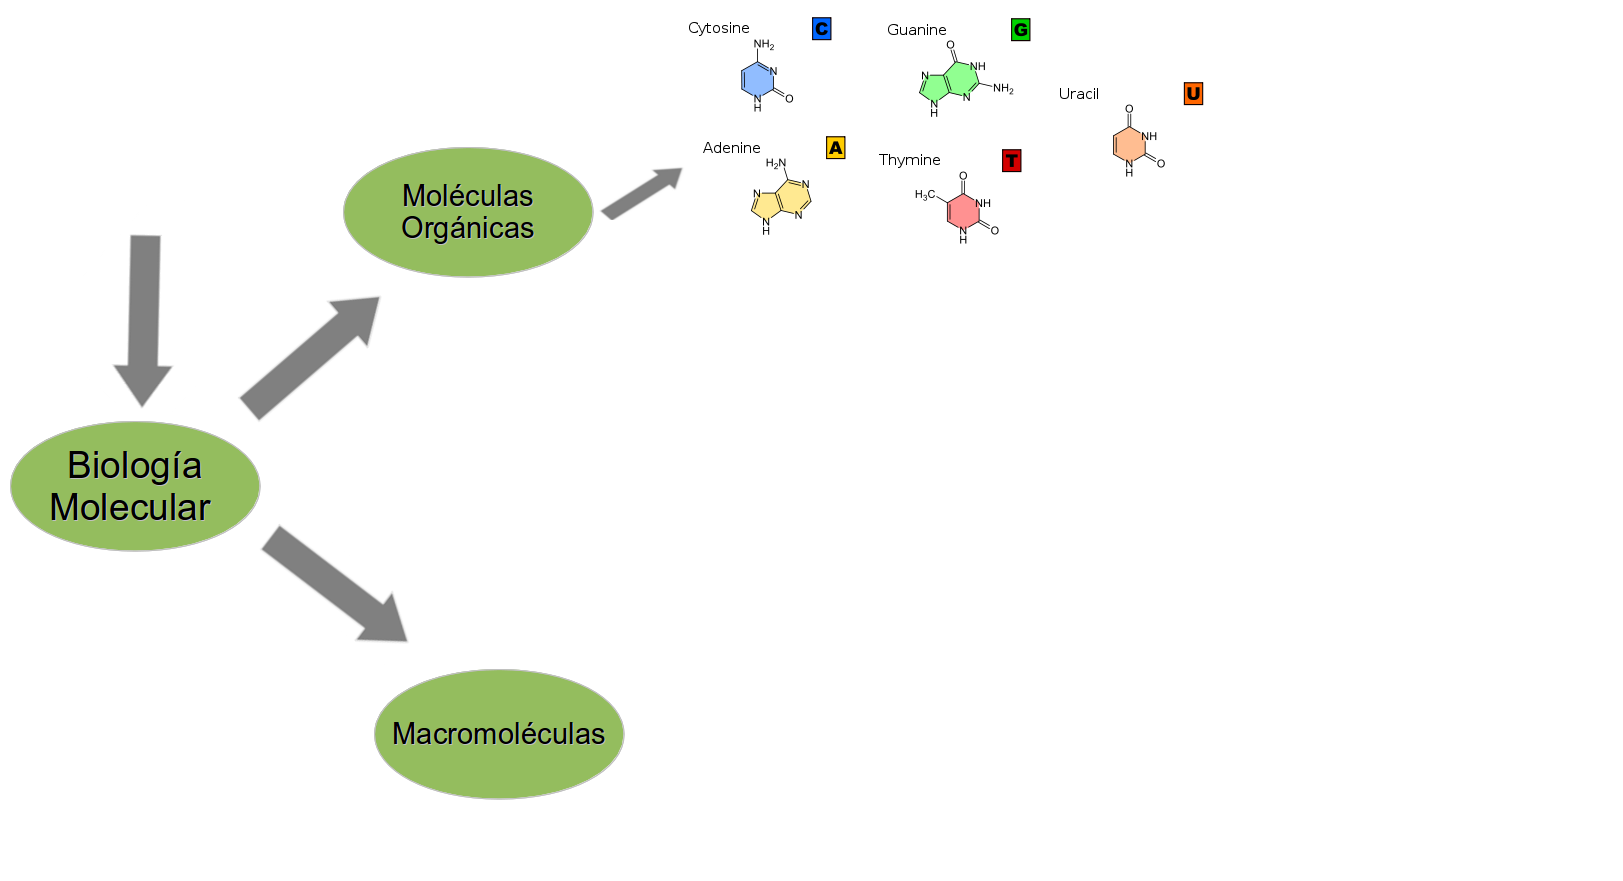
\includegraphics[scale=.2]{images/biologia3.png}
        \end{center}
    \end{frame}
    
    \begin{frame}\frametitle{\textbf{Conceptos de Biología}}
        \begin{center}
          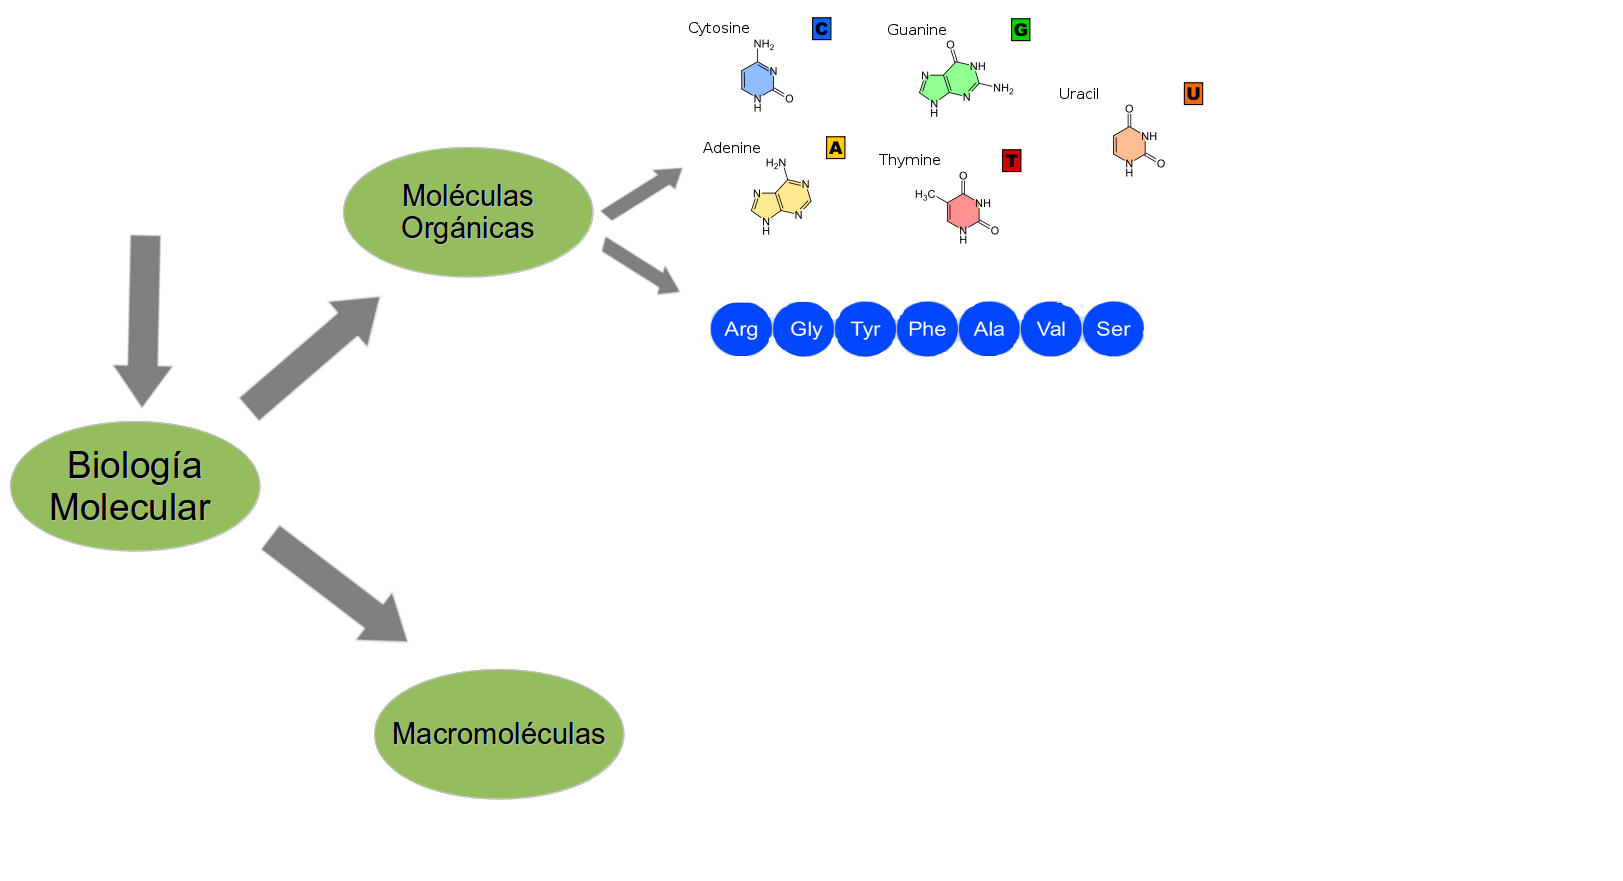
\includegraphics[scale=.2]{images/biologia4.png}
        \end{center}
    \end{frame}

    \begin{frame}\frametitle{\textbf{Conceptos de Biología}}
        \begin{center}
          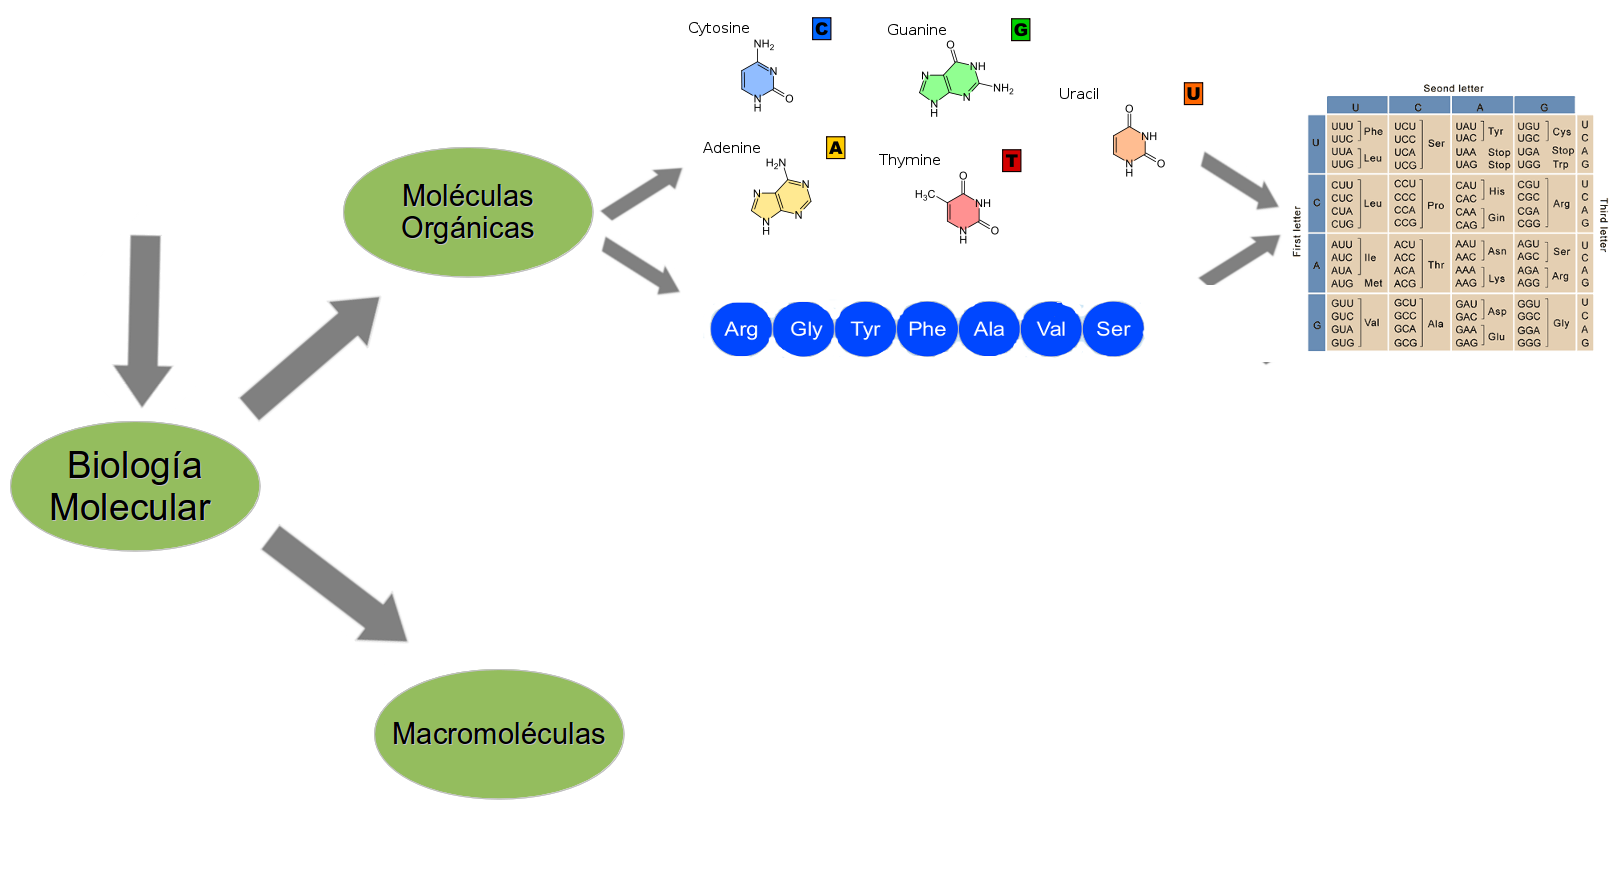
\includegraphics[scale=.2]{images/biologia5.png}
        \end{center}
    \end{frame}

    \begin{frame}\frametitle{\textbf{Conceptos de Biología}}  
        \begin{center}
          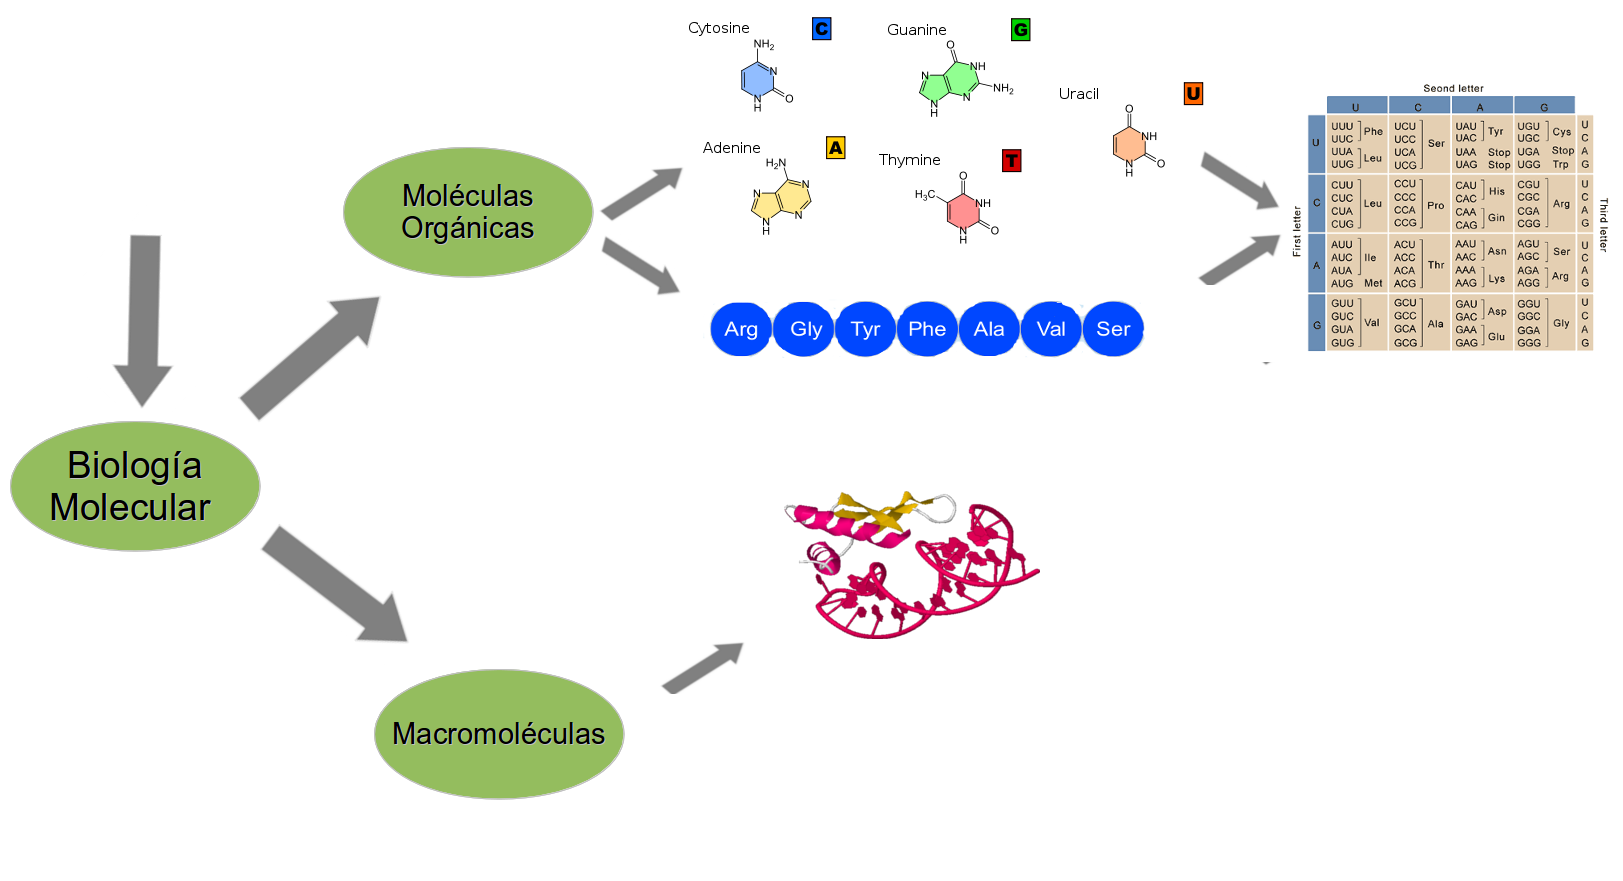
\includegraphics[scale=.2]{images/biologia6.png}
        \end{center}
    \end{frame}

    \begin{frame}\frametitle{\textbf{Conceptos de Biología}}
        \begin{center}
          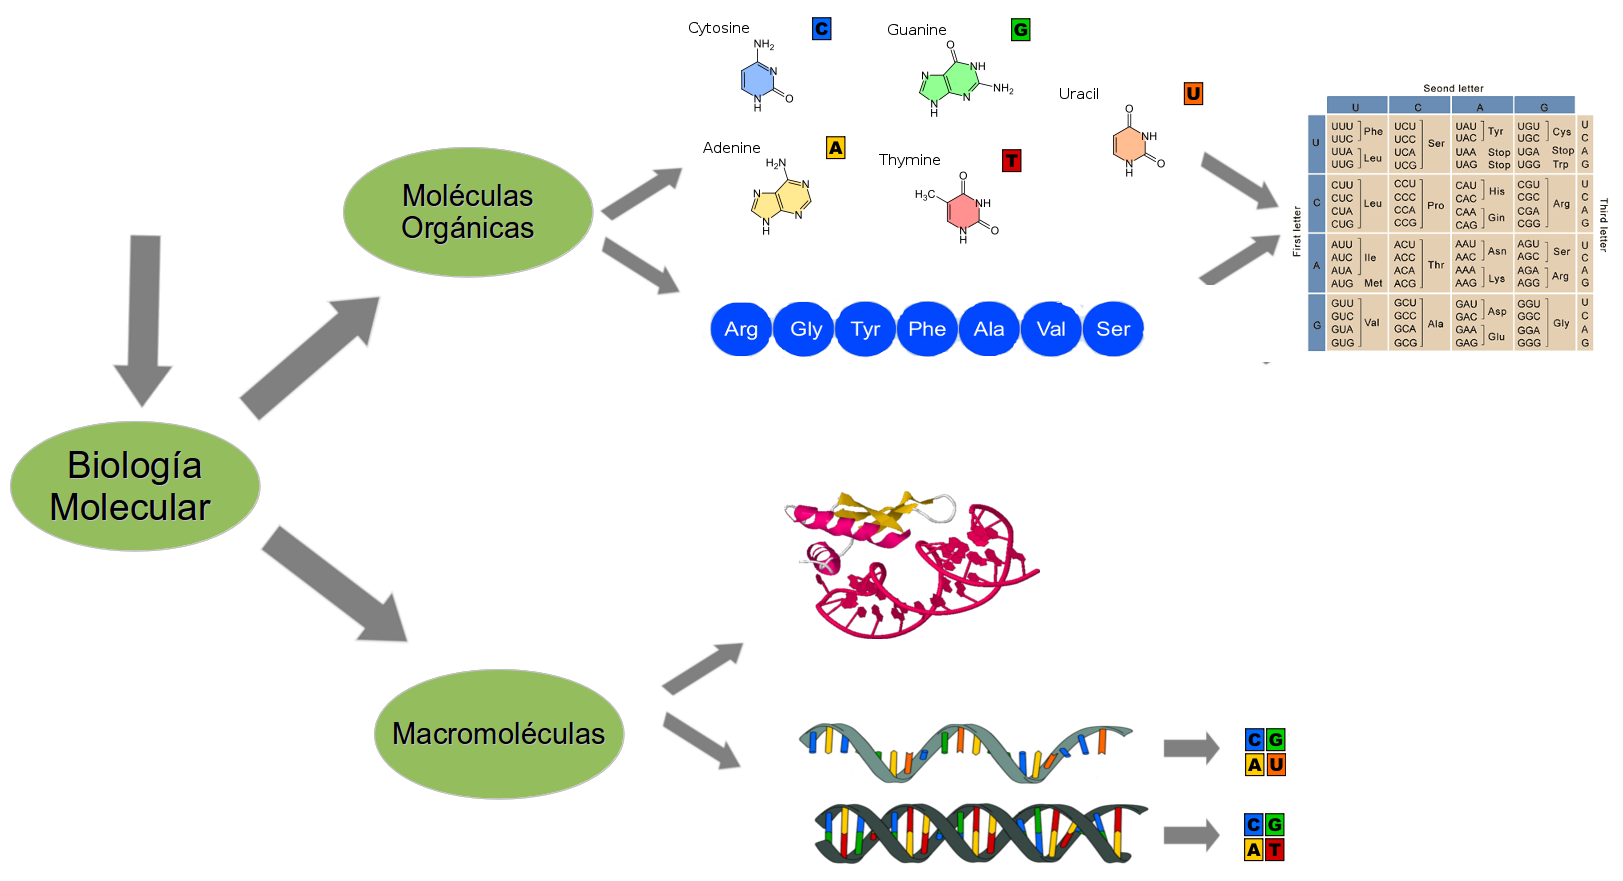
\includegraphics[scale=.2]{images/biologia7.png}
        \end{center}
    \end{frame}

    \begin{frame}\frametitle{\textbf{Ácidos Nucleícos}}
      \begin{block}{}
        \begin{center}
          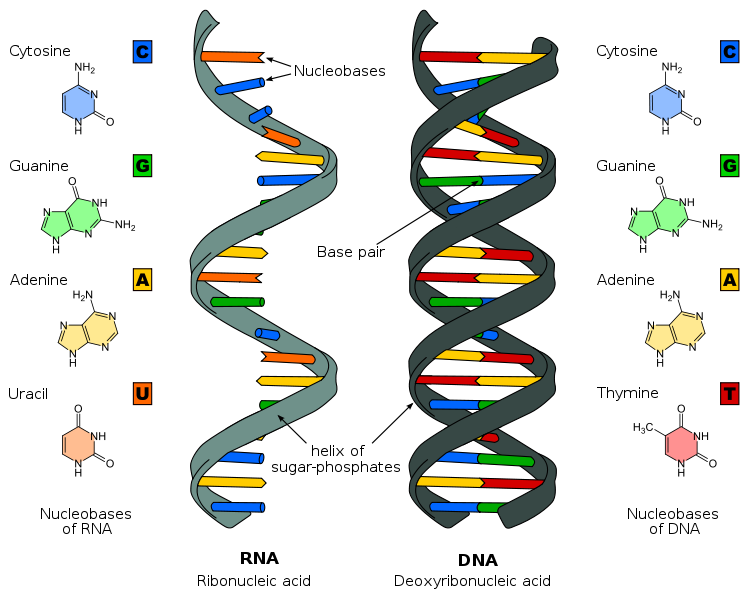
\includegraphics[scale=.3]{images/adnrna.png}
        \end{center}
      \end{block}
    \end{frame}

    \begin{frame}\frametitle{\textbf{Ácidos Nucleícos (cont.)}}
      \begin{block}{RNA}
        \begin{figure}[h]
          \begin{minipage}{0.7 \textwidth} 
            Generalmente, consiste en una hebra de cadena simple, la cual usualmente es trascripta a partir de una porci\'on de ADN y se utiliza posteriormente en la c\'elula para la s\'intesis de prote\'inas. Algunos virus poseen ARN como \'unico material gen\'etico cuya monohebra puede plegarse, dando lugar a lo que se conoce como estructura secundaria.
          \end{minipage}
          \begin{minipage}{3cm}
          \begin{center}
           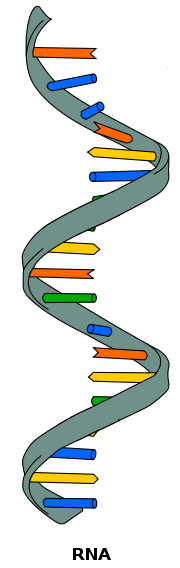
\includegraphics[scale=.15]{images/rna.png}
          \end{center}
          \end{minipage}
        \end{figure}
      \end{block}

      \begin{block}{La Estructura Primaria y Secundaria del RNA}
        La estructura primaria del ARN, es una secuencia de nucle\'otidos de longitud $n$, $A=a_{1}a_{2}a_{3}\dots a_{n}$ con $a_{i} \in \left\lbrace A, U, G, C \right\rbrace$. El plegamiento de una secuencia de ARN entre sus bases complementarias determina lo que se denomina estructura secundaria de ARN.
      \end{block}
    \end{frame}

    \begin{frame}\frametitle{\textbf{Estructura Secundaria del RNA (motifs)}}
        \begin{center}
          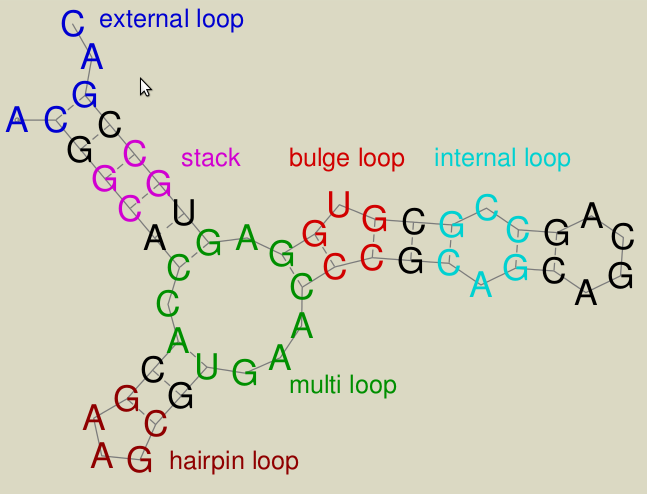
\includegraphics[scale=.38]{images/rnaMotifs.png}
        \end{center}       
    \end{frame}

    \begin{frame}\frametitle{\textbf{Estructura Secundaria del RNA (cont.)}}
        \begin{center}
          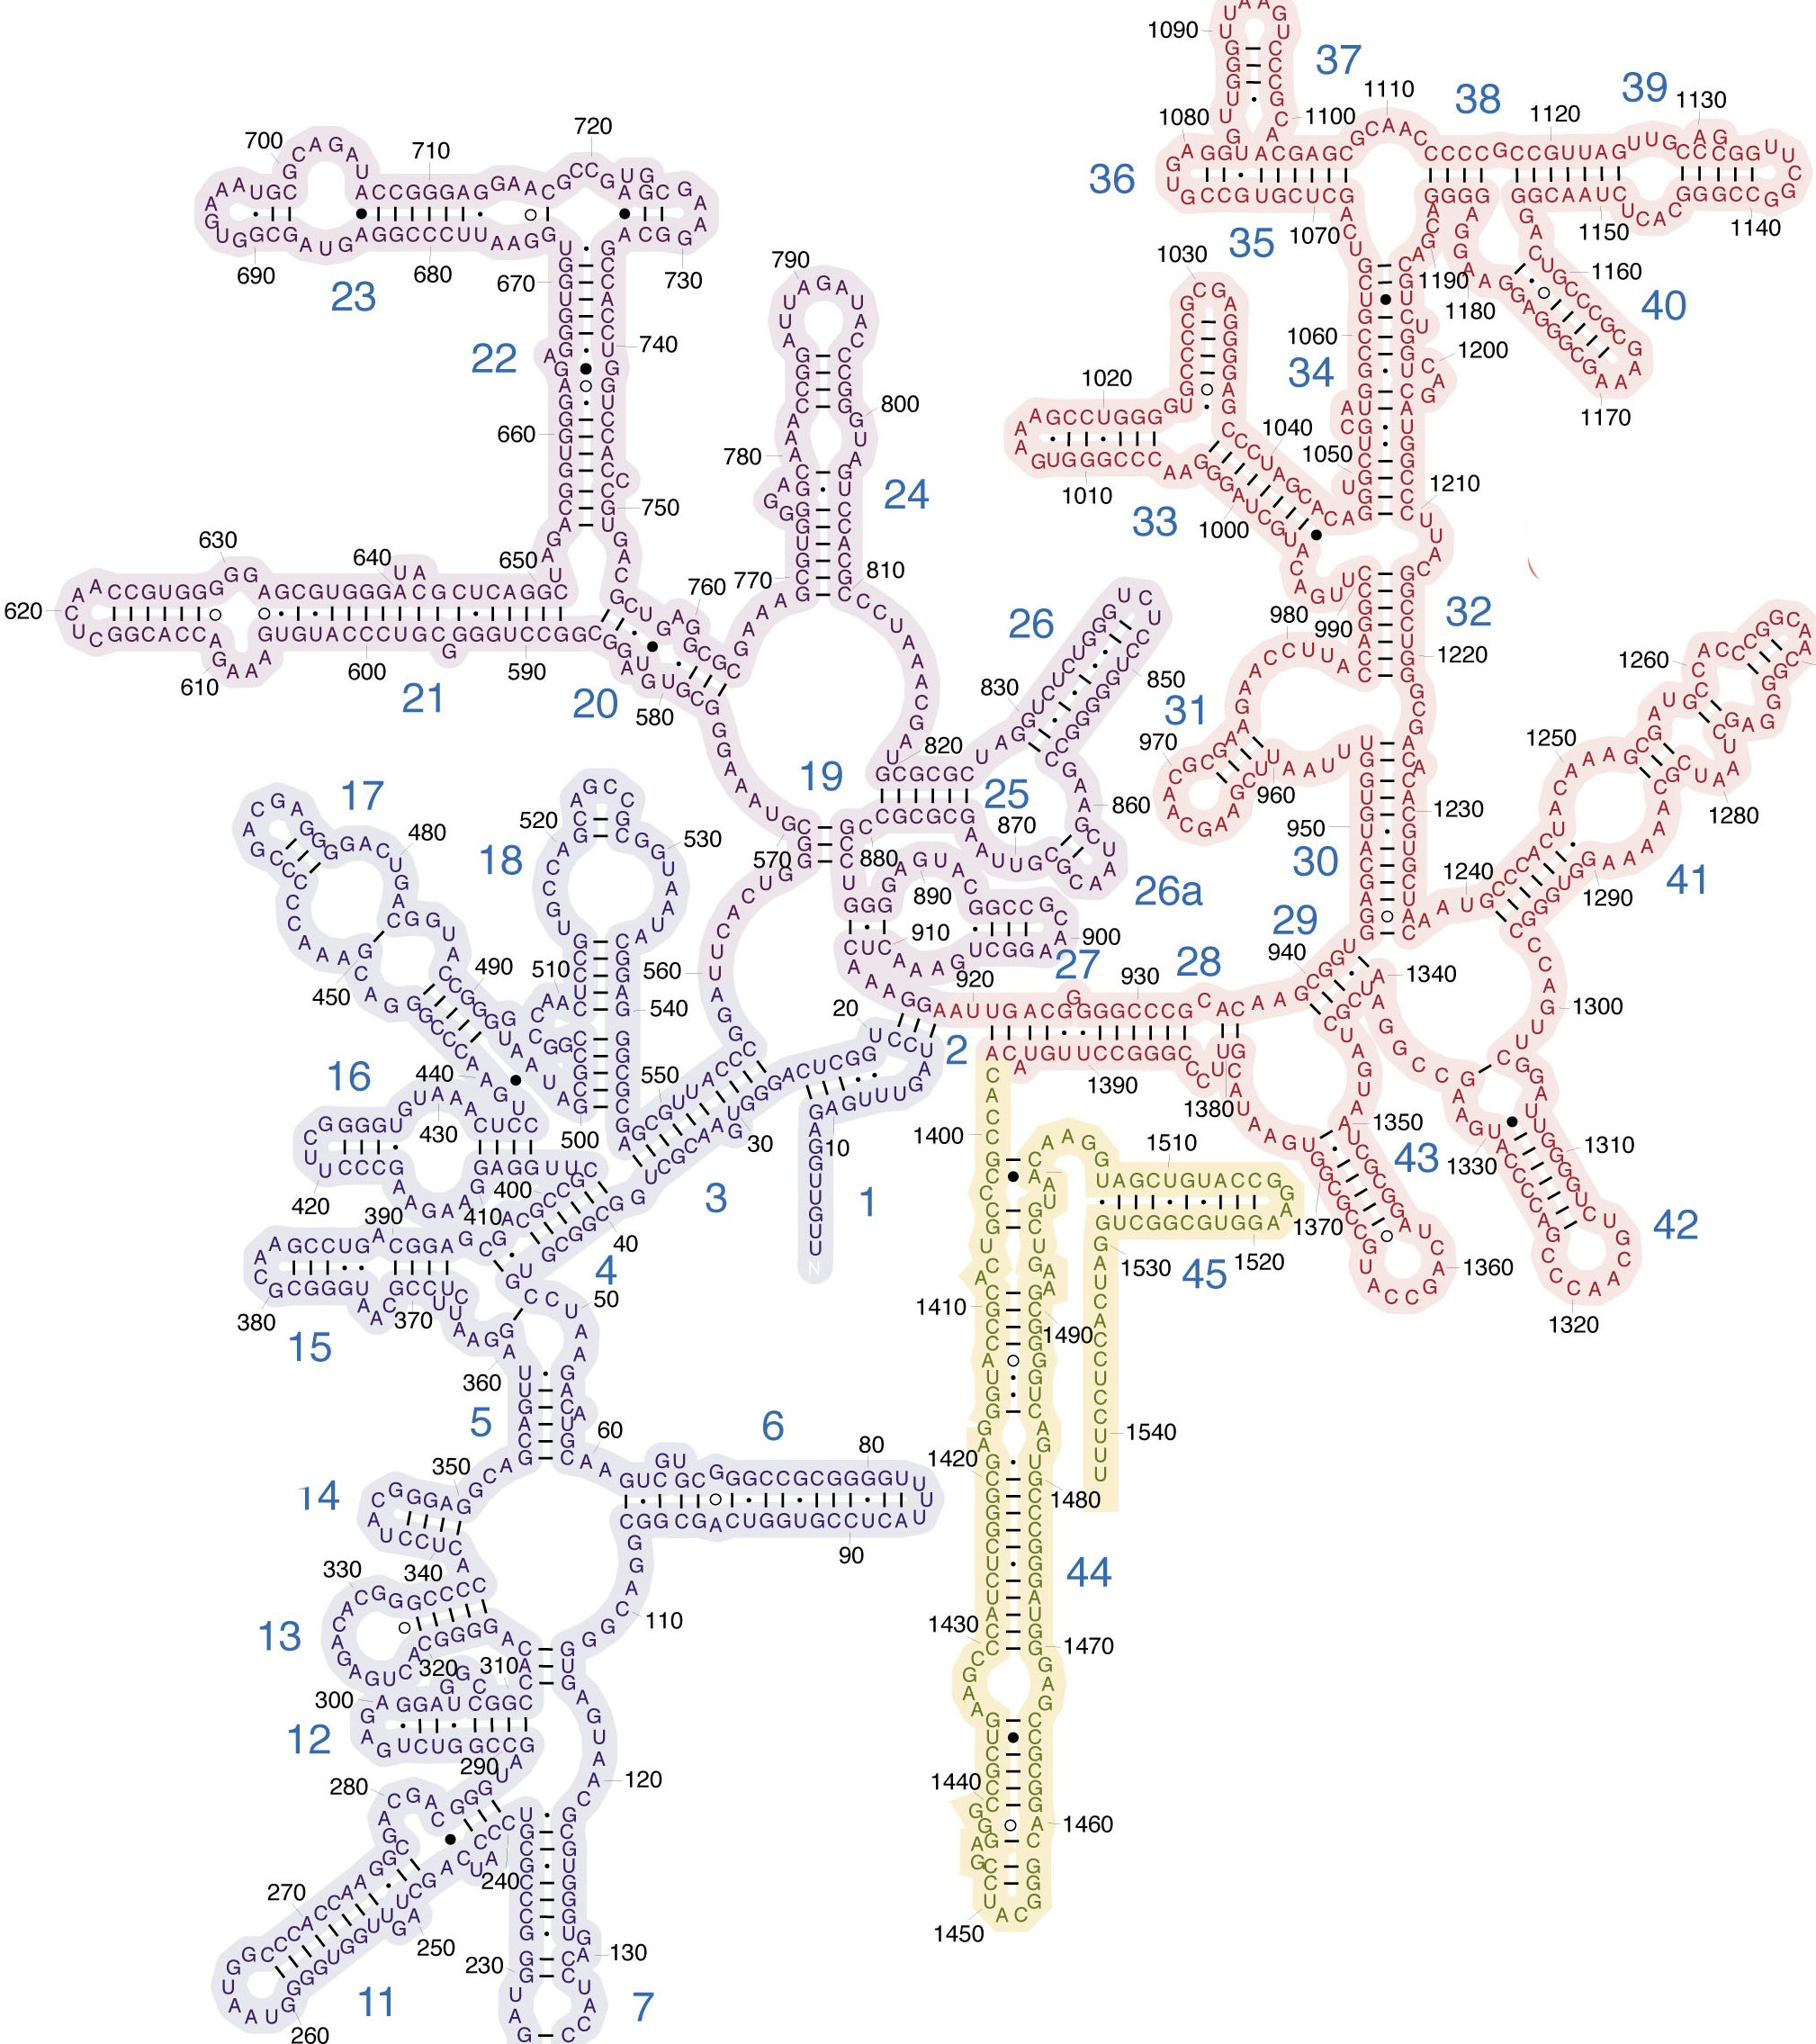
\includegraphics[scale=.39, angle=90]{images/complex.jpg}
        \end{center}       
    \end{frame}

    \begin{frame}\frametitle{\textbf{Dogma Central de la Biología}}
        \begin{center}
          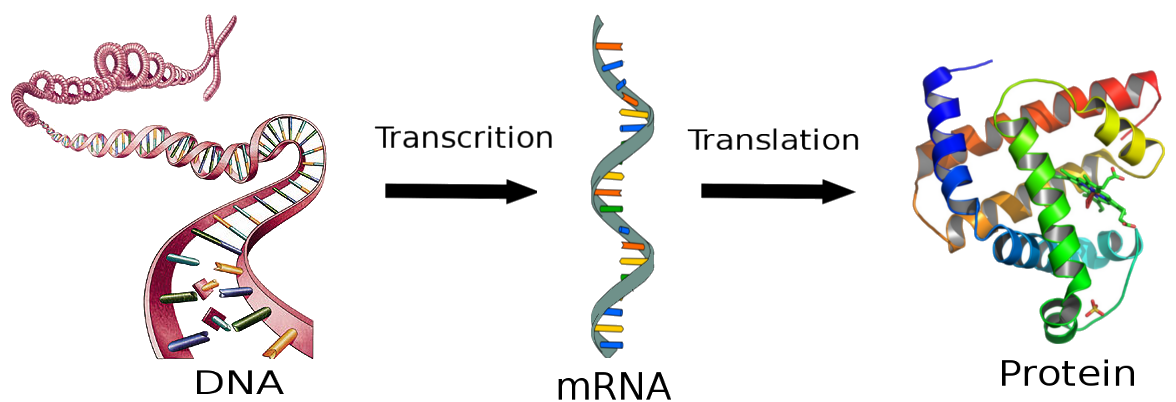
\includegraphics[scale=.26]{images/centralDogma.png}
        \end{center}       
    \end{frame}
